Form the preceding section, probably the reader has envisioned already the dots to connect from both ingredients, the Gaussian process implicit surfaces and the AtlasRRT methodology. The next paragraphs formally describes these connections as the GPAtlasRRT strategy, to give one possible answer to the question raised in the problem statement: an strategy that suggest the best-next tactile exploration candidates to improve the object surface representation, exploiting its probabilistic nature. 

The method starts from an initial and partial observations of the object surface. This is generally provided by vision due to its ability to cope with several points at once. To this end, we assume there is a way to segment the object points out of the scene, that is, points on the object surface\footnote{We provide technical details of our implementation in a real scenario in Subsection~\ref{sec:real}}. However, there could be no information at all, and the probe naively go towards the palm of the gripper holding the object to get a first initial observation, and start from there. As one would expect, this increases the time to get an accurate shape. This initial observations go directly to form the set $\mathcal{S}^0$ to have the object surface model, $\mathcal{GP}$, model provided by (\ref{eq:gp_model}). Since these points are axiomatically on the surface with some degree of uncertainty due the sensor noise, we can compute charts on each of them.
Algorithm \ref{alg:strategy} describes the next-best candidate points for a tactile exploration that to improves input model, $\mathcal{GP}$, up to a predefined variance, $\mathbb{V}_{\max}$. 
The first thing to do is to \textsc{selectSurfacePoint} (line \ref{init}) randomly to get a point $\mathbf{x}_i \in \mathcal{X} \subset \mathcal{S}^0$\footnote{In theory, we can start from all points in the surface, but in practice, this requires too many multi-processes to be properly synchronized}. This is the starting point where the first chart is created, invoking the \textsc{createChart} function (line \ref{create_chart}). The generated data structure contains the center, $\mathbf{x}_i$, the orthonormal tangent basis provided by (\ref{eq:tangent_basis}), $\boldsymbol{\Phi}_i$, note that $\nabla f(\mathbf{x})$ is equivalent to (\ref{eq:gradient_f}), its size, $\rho_i$, and a set of points in the tangent space, $\mathcal{U}_i$. Two things are noticeable here that differentiate us from the original AtlasRRT algorithm. Firstly, the size of a chart, which is a similar to the validity region notion, is inversely proportional to the variance at the chart center, namely,
\begin{equation}
\rho_i \propto \mathbb{V}[f(\mathbf{x}_i)]^{-1}.
\end{equation}
This size is actually the radius of a ball centered at $\mathbf{x}_i$, whose intersection with the tangent space yields \emph{disk}. The motivation behind this choice is that the more certain a point is to be on the surface, the larger the covered region of its chart on the predicted shape, whereas the more uncertain is associated to the center, we prefer to perform smaller exploratory steps.
And secondly, a number proportional to the size of points are sampled uniformly and randomly in the annulus region of the disk with internal and external radius being $0.8\rho$ and $\rho$, respectively. The cardinality of this point-set in the tangent space is proportionally to its size, namely,
\begin{equation}
\#\mathcal{U}_i \propto \rho_i.
\end{equation}
This leads to the fact that the larger the chart, the higher the resolution of directions to expand, hence more samples are needed to have a good quantization of it.
Another advantage of working with a normalized and offset-free set, as mentioned in Subsection \ref{sec:gpis}, is that the parameters that makes the latter two expression to be equalities are tuned once, and remain fixed.

\begin{algorithm}[t]
    \textbf{$\mathcal{P} \leftarrow$ \textsc{GPAtlasRRT}}($\mathcal{M}$, $\mathbb{V}_{\max}$)\\ %functionname
\LinesNumbered
\DontPrintSemicolon
\SetAlgoVlined \SetKwInOut{Input}{input} \SetKwInOut{Output}{output}
\Input{A Gaussian Process model, $\mathcal{M}$ and the set of parameters $\Omega$, defining criteria
    to decide how to start, extend and end the exploration.}
\Output{The best next action, $\mathcal{P}$, in the form of a path, if any, or $\varnothing$ otherwise.}
$\mathbf{x_i} \leftarrow$ \textsc{selectSurfacePoint}($\mathcal{GP}$) \label{init} \\ 
$\mathcal{C}_{i} \leftarrow$\textsc{createChart}($\mathbf{x}_i$, $\mathcal{GP}$) \label{create_chart} \\
% $\mathcal{A}, \mathcal{T}, \mathbf{x}_{c,i} \leftarrow$\textsc{init}($\mathcal{M}$, $\Omega$) \\
$\mathcal{A} \leftarrow$ \textsc{addChart}($\mathcal{C}_i$) \label{add_chart} \\
  \label{is_expandable} \While{ \textsc{isExpandable}($\mathcal{A}$) }
  {
    $\mathcal{C}_j \leftarrow$\textsc{selectChart}($\mathcal{A}$) \label{select_chart} \\
    $\mathbf{x}_k \leftarrow$\textsc{expandChart}($\mathcal{C}_j$, $\mathcal{GP}$) \label{expand_chart} \\
    $\mathcal{C}_k \leftarrow$ \textsc{createChart}($\mathbf{x}_k$, $\mathcal{GP}$) \label{create_new_chart} \\
    $\mathcal{A} \leftarrow$\textsc{addChart}($\mathcal{A}$, $\mathcal{C}_k$) \label{add_new_chart} \\
    \label{ending} \If{ $\mathbb{V}[f(\mathbf{x}_k)]  > \mathbb{V}_{\max}$ }
    {
      $\mathcal{P} \leftarrow$ \textsc{getPath}($\mathcal{C}_i$, $\mathcal{C}_k$) \label{compute_path} \\
      \Return $\mathcal{P}$ \label{return_path} \\
    }
    % \textsc{connect}($\mathcal{T}$, $\mathcal{C}_{k}$, $\mathcal{C}_{j}$) \\
    %$\mathcal{C}_{i} = \mathcal{C}_{k}$ \\
  }
  %\eIf {\textsc{solution}($\mathcal{C}_{i}$)}
  %{\Return $\mathcal{P} \leftarrow$\textsc{path}($\mathcal{C}_{i}, \mathcal{T}$)}
  \Return $\varnothing$ \label{no_candidate}
  \caption{The GPAtlasRRT strategy} \label{alg:strategy}
\end{algorithm}

\begin{figure*}
    \centering
    \mbox
    {
        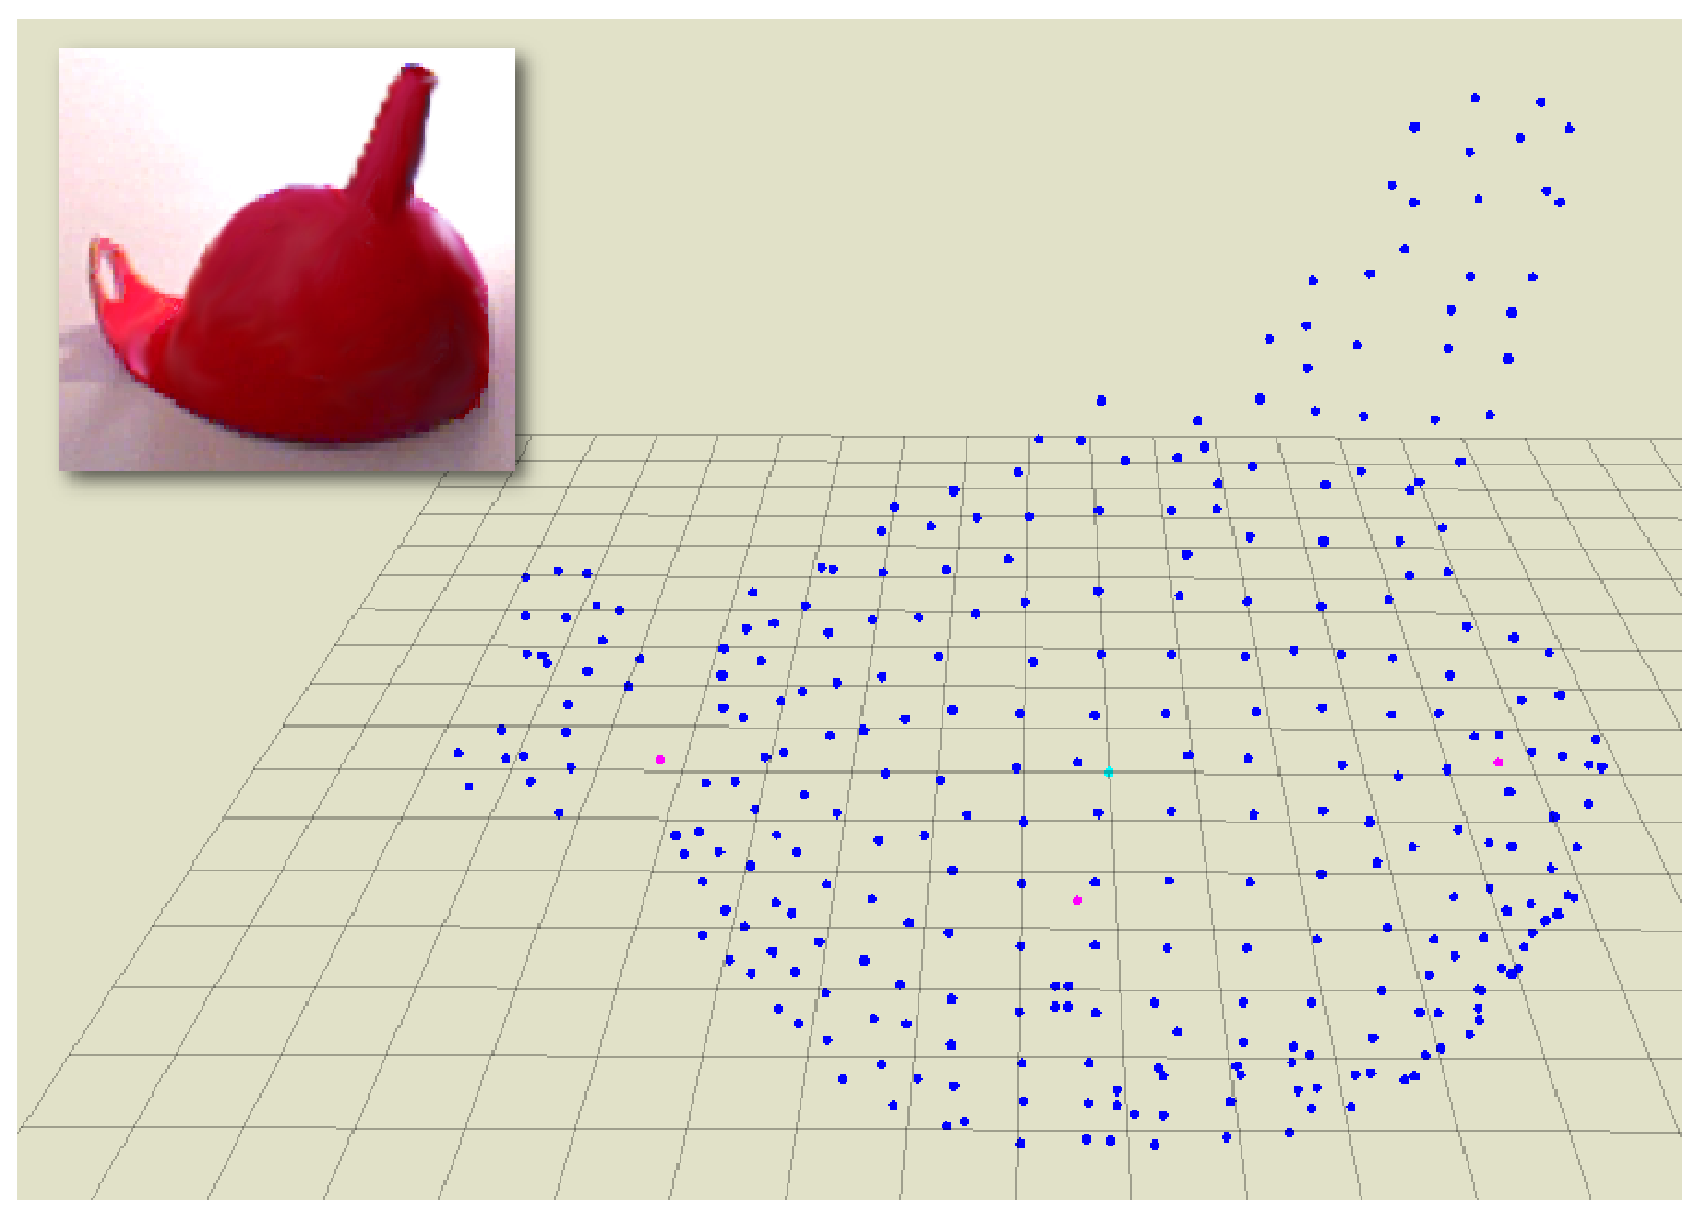
\includegraphics[width=0.33\linewidth]{funnelC.eps}
        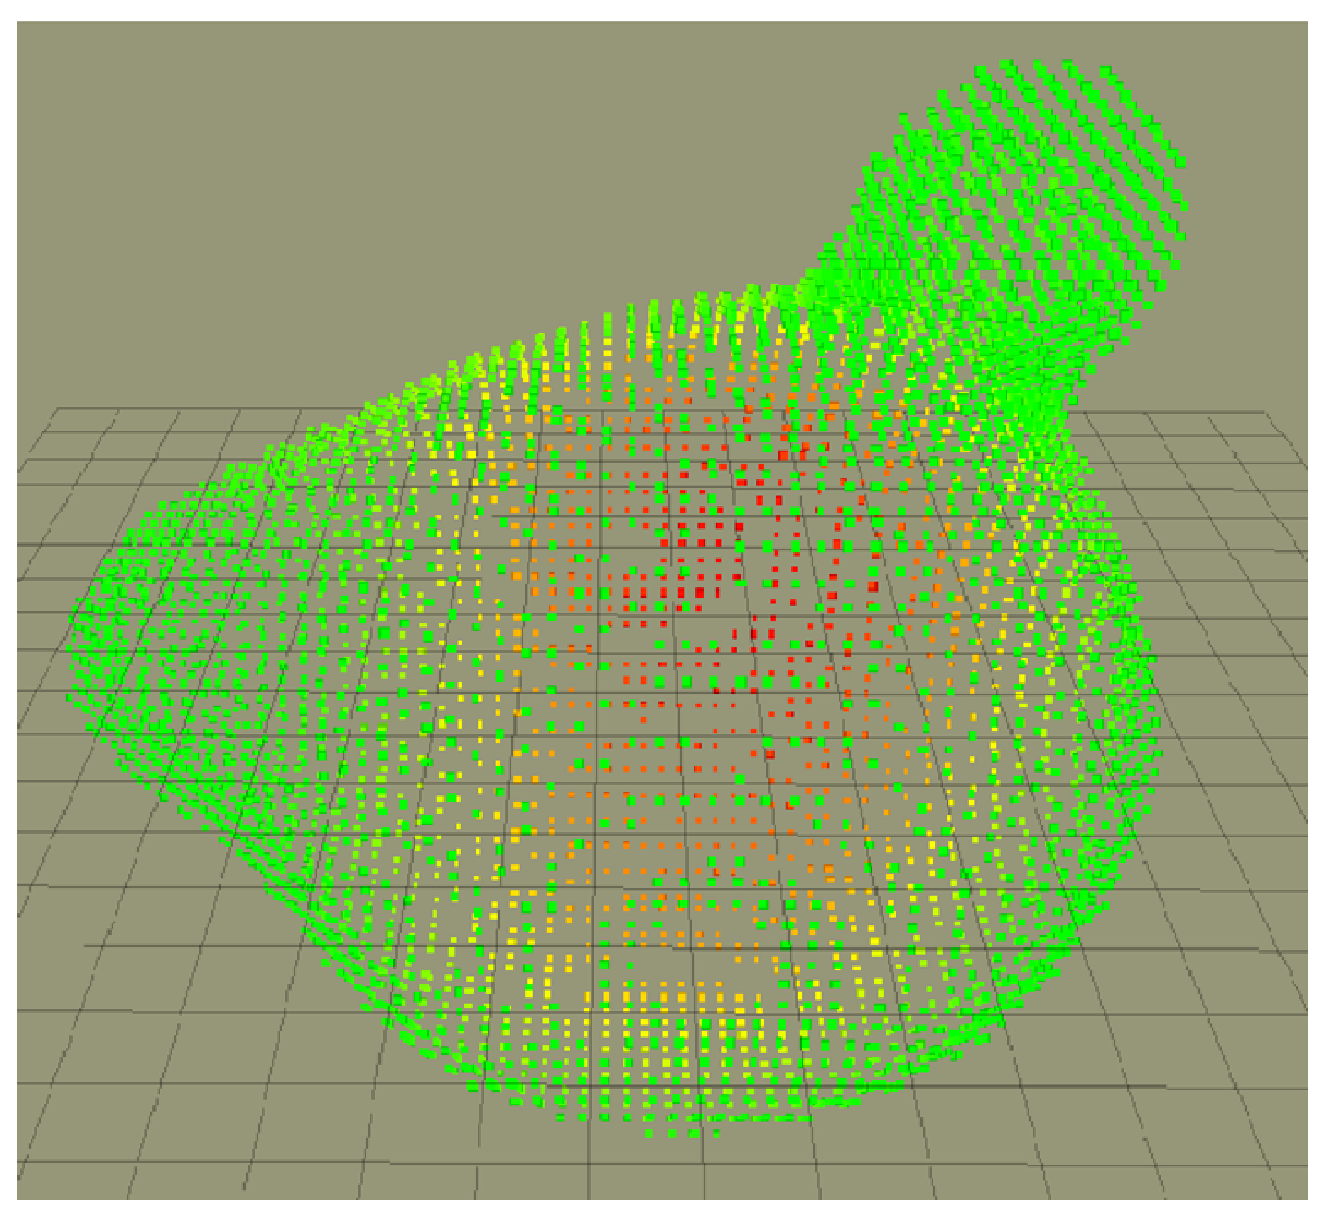
\includegraphics[width=0.33\linewidth]{funnelS.eps}
        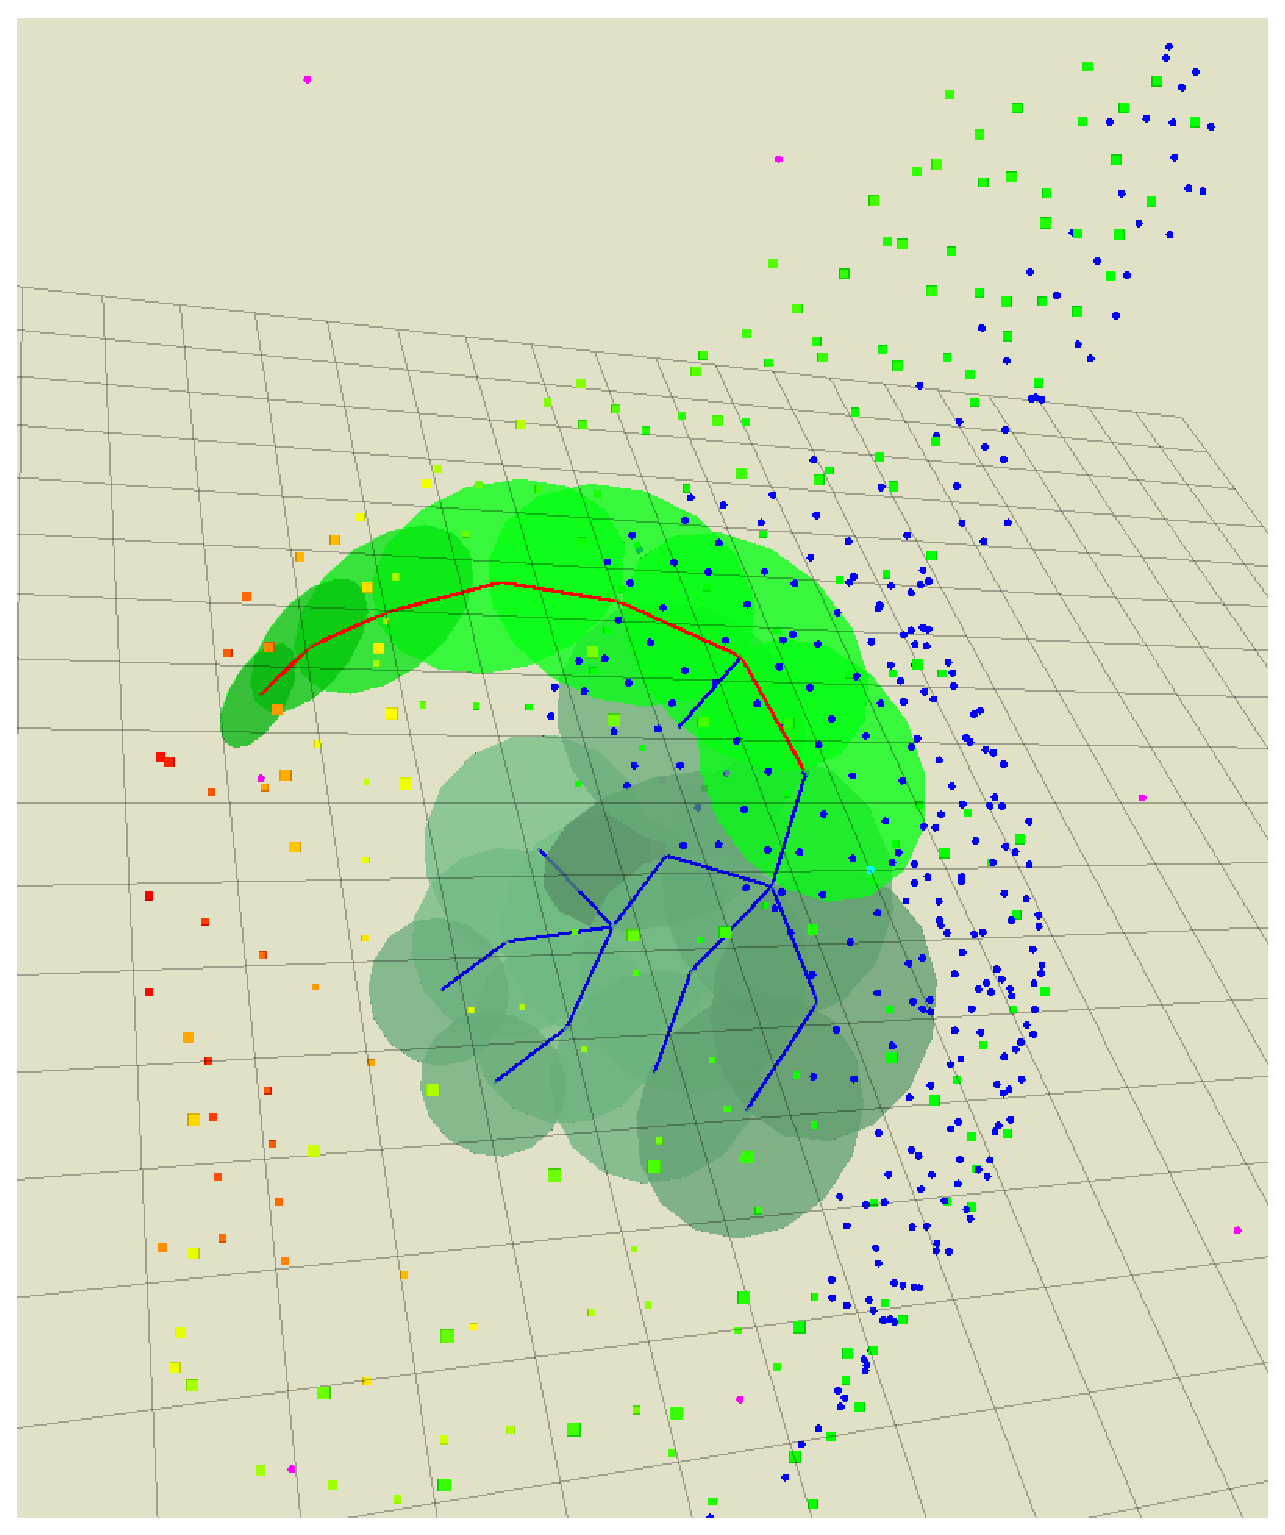
\includegraphics[width=0.33\linewidth]{funnelRRT.eps}
    }
    \caption{ A funnel (left-upper corner) is first seen by a depth camera. The segmented 3D points are sown in blue in the left figure to form the training set $\mathcal{S}^0$. The predicted shape by the GP on this set is shown in the middle obtained via the marching cube algorithm. However, the GPAtlasRRT strategy does not require the explicit form of the predicted surface, as shown in the right figure. It works with the implicit form to devise the next-best tactile exploration shown in brighter green.}
    \label{fig:GPAtlasRRTfunnel}
\end{figure*}

The algorithm continues with the addition of this first chart to the atlas, $\mathcal{A}$, that becomes the root node of an exploration tree (line \ref{add_chart}). The question whether an atlas \textsc{isExpandable} or not (line \ref{is_expandable}) is readily answered by checking whether there is at least one chart with $\#\mathcal{U}_j \neq 0$ or not. The \texttt{false} condition implies that we have covered completely the predicted surface, exiting with no candidate for the best-next tactile exploration (line \ref{no_candidate}). The \texttt{true} condition then makes the flow to continue within the \textbf{while} loop for the iterative exploration. The first step is to \textsc{selectChart} (line \ref{select_chart}) to expand from the atlas. This action takes place randomly among all current charts whose point-set $\mathcal{U} \neq \emptyset$ using a trade-off proportion between depth-first (or selecting the previously expanded chart with probability $p = 0.4$) and breadth-first (or selecting any other chart with probability $1-p$) for the tree expansion. Note that, in the first iteration, $\mathcal{C}_i$ is the only one, and it is surely expandable. Next, the \textsc{expandChart} operation on the selected chart (line \ref{expand_chart}) chooses among all points $\mathbf{u}_{j,t} \in \mathcal{U}_i$, the one with the largest variance in ambient space, that is,
\begin{equation}
\mathbf{u}_{j}^* =  \argmax_{\mathbf{u}_{j} \in \mathcal{U}} \mathbb{V}[f(\phi_j(\mathbf{u}_{j}))], 
\end{equation}
where the tangent basis approximation of the mapping $\phi_j(\cdot)$ is used as given in (\ref{eq:tangent_approx}). The point $\mathbf{x}_k^j = \phi(\mathbf{u}_{j}^*)$ is then projected to the predicted surface solving (\ref{eq:projection}), as mentioned, using a gradient-descent-like method to obtain the point $\mathbf{x}_k \in \mathbf{X}$. A chart, $\mathcal{C}_k$, is then created from this point and added to the current atlas (lines \ref{create_new_chart}--\ref{add_new_chart}). When a new chart is added to the atlas, all sets $\mathcal{U}$ of all charts are reduced by discarding the points that fall within the validity region of other charts existing in the atlas. This was not mentioned in the first call of the \textsc{addChart} in line \ref{add_chart}, because at that point there is only the root chart in the atlas. Finally, the expected variance of the center of the last chart added is compared against the input parameter $\mathbb{V}_{\max}$ (line \ref{ending}). The \texttt{false} condition of the \textbf{if} statement makes the algorithm to continue with the atlas expansion, whereas the \texttt{true} condition return the next-best exploration path, $\mathcal{P}$ (lines \ref{compute_path}--\ref{return_path}). Recall that this path is in the predicted shape of the object, therefore the control to follow it must be compliant to avoid damages. The new tactile observations tells whether the predicted shape is good or not by increasing the training set, $\mathcal{S}^0$, to automatically reduce the variance along the path, and improve the overall uncertainty of surface model. The next section traces how the GPAtlasRRT strategy can be embedded in a tactile exploration scenario.

\subsection{Tactile exploration for object surface modeling via the GPAtlasRRT strategy}
\label{sec:gpatlasrrt_tactile_exploration}

Algorithm~\ref{alg:solution} presents the pipeline model of a tactile exploration to model the surface of an object driven by the GPAtlasRRT strategy. As anticipated in the previous section, the initial and partial observation can be taken from visual input or a naive probe (lines to compute the model \ref{ini_gp}--\ref{fini_ini_gp}). From this point on, we plan the next-best tactile exploration, $\mathcal{P}$, (line \ref{exploration}), and pass this information to the exploratory probe. Please, note that this exploration can done by a real robot or simulated given a ground truth, a notion that is used for the method validation in Section \ref{sec:experiments}.

Thus, the exploratory probe system \textsc{approachTo} the exploration path, typically to the first point with low uncertainty when \emph{sliding} or to the final point with high uncertainty when \emph{poking} with the goal being a safety distance away from the predicted surface in the direction normal at the corresponding point. This phase can be done with a position control scheme and collision avoidance motion planning. The latter is an interesting topic, since the object shape is not known. But it can be predicted with the current state of the model to some degree of uncertainty. A coarse point cloud can be computed out of the model and build a probabilistic collision map based on the expected variance of the function values at the point cloud. Next, we proceed to \textsc{probeObject} following the next-best path, $\mathcal{P}$, to get observations of points being on or outside of the surface, and labeled accordingly altogether in the exploration log set, $\mathcal{S}^{0+}$ (line \ref{probe}). In this phase, the collision avoidance motion is disable and the probe moves compliantly, like in a contour-following set-up, and uses the tactile sensing to detect whether the probe is contacting or not with the object surface. Once the end of the path is reached, the training set is accordingly updated keeping the old training set, and applying the normalization and offset-free operations after the addition of new data (line \ref{update_training}). This is then used to recompute a better model of the object surface, $\mathcal{GP}$ (line \ref{re-compute}). Simultaneously (using the old model) or afterwards (using the updated model), we engage again the position control and collision avoidance motion planning to take the exploratory probe to its rest position (line \ref{away}). When the \textsc{GPAtlasRRT} returns an empty path, $\mathcal{P} = \varnothing$, then we say that the predicted shape by the returned model, $\mathcal{GP}$, has at most a variance of $\mathbb{V}_{\max}$ for any point on the surface, that is, $\mathbb{V}[f(\mathbf{x})] < \mathbb{V}_{\max}, \, \forall \mathbf{x} \in \mathcal{X}$.

\begin{algorithm}[t]
\textbf{\textsc{TactileExploration}}($\mathcal{Z}, \mathbb{V}_{\max})$\\ %functionname
\LinesNumbered
\DontPrintSemicolon
\SetAlgoVlined \SetKwInOut{Input}{input} \SetKwInOut{Output}{output}
\Input{An initial point cloud of the scene, $\mathcal{Z}$, and the desired variance, $\mathbb{V}_{\max}$, for the overall surface prediction.}
\Output{The object model as a Gaussian process, $\mathcal{GP}$.}
  \label{ini_gp} \If{ \textsc{isEmpty}($\mathcal{Z}$ }
  {
    $\mathcal{S}^0 \leftarrow $ \textsc{naiveProbe}() \\
  }
  \Else
  {
    $\mathcal{S}^0 \leftarrow $ \textsc{segmentObject}($\mathcal{Z}$) \\
  }
  $\mathcal{S} \leftarrow$ \textsc{generateTrainSet}($\mathcal{S}^0$)
  $\mathcal{GP} \leftarrow $\textsc{computeModel}($\mathcal{S}$) \label{fini_ini_gp} \\
  \While { \texttt{true} } 
  {
    $\mathcal{P} \leftarrow $\textsc{GPAtlasRRT}($\mathcal{GP}, \mathbb{V}_{\max})$ \label{exploration} \\
    \If{ $\mathcal{P} \neq \varnothing$ }
    {
      \textsc{ApproachTo}($\mathcal{P}$, $\mathcal{GP}$) \label{approach} \\
      $\mathcal{S}^{0+} \leftarrow $\textsc{probeObject}($\mathcal{P}$) \label{probe} \\
      %$\mathcal{S}^0 \leftarrow$ \textsc{getOnSurface}($\tilde{\mathcal{S}^{0+}}$) \\
      %$\mathcal{S}^+ \leftarrow$ \textsc{getOutsideSurface}($\tilde{\mathcal{S}^{0+}}$) \\
      $\mathcal{S} \leftarrow$ \textsc{updateTrainSet($\mathcal{S}$, $\mathcal{S}^{0+}$)} \label{update_training} \\
      $\mathcal{GP} \leftarrow $\textsc{computeModel}($\mathcal{S}$) \label{re-compute} \\
      \textsc{MoveAway}($\mathcal{GP}$) \label{away} \\
    }
    \Else
    { 
      \Return {$\mathcal{GP}$} \label{solutionfound} \\
    }
  }
\caption{Surface modeling via GPAtlasRRT} \label{alg:solution}
\end{algorithm}

%\subsection{Probabilistic completeness}
%\label{sec:reasoning}

%First of all, we can safely assume that the surface of any household object is a $1$-component manifold.








% During the \textsc{ApproachTo} (line~\ref{approach}) (\textsc{MoveAway}, line~\ref{away}) phases, the robot uses position control and standard motion planning techniques with collision avoidance. Since we are modelling the shape, we need to ensure that everytime the robot moves close (away) from the object, it does not collide with the object. It is tentative to use the current estimated shape, but since we are not actually computing it explicitly in our approach, we choose the bounding sphere as the collision geometry of the object. Thus the robot moves towards (away from) the surface at the contact location in the normal direction until reaching the bounding sphere. After that, a standard motion planning is used to approach the object (get to the rest position).

% The \textsc{probeObject} (line~\ref{probe}) phase is engaged once the robot is within the bounding sphere. The robot uses Cartesian impedance control, with the Cartesian force, pose and impedance set properly for the given setup. These implementation details are given in the next section. Since we don't actually know where the surface is, we need to whether the robot actually touched something or not, in order to properly label the acquisition (lines~\ref{belonglabel} and~\ref{nobelonglabel}) 

% The method finishes when \textsc{exploreGPAtlasRRT} (line~\ref{exploration}) described in Algorithm~\ref{algo:strategy} has explore sufficiently the estimated shape and could not find an exploratory action $\Gamma$ (line~\ref{solutionfound}), i.e. the object shape is probabilistically estimated within the 95\% of the confidence interval computed from $\mathbb{V}_{des}$. 

%The complete solution of the problem as stated in~\ref{sec:scope} is depicted in Algorithm~\ref{alg:solution}.



%This section provides a more detailed description of our GPAtlasRRT algorithm. As described in Sec.~\ref{sec:scope}, our approach combines probabilistic inference on an unknown surface with a asymptotically optimal sample-based exploration technique for implicitly-defined configuration spaces (manifolds). We demonstrate the efficiency of our proposed solution in a bimanual framework (see Sec.~\ref{sec:scenario}) where a humanoid robot (Vito) can hold an unknown object in one hand and actively build up a probabilistic model of the object's shape by integrating visual and haptic information. This is done efficiently by selecting haptic actions which lead to an asymptotically optimal reduction of the global shape uncertainty of the model. 

%We employ a GP to learn a probabilistic model of the object surface, encoded as an implicit surface, constrained to visual and tactile clues iteratively acquired. First we rely on visual information captured by a RGB-D camera, which will be pre-processed, as described in Sec.~\ref{sec:segmentation}, to isolate the object's point cloud from the rest of the scene (robot's and environment's). Secondly we generate artificial points to improve the performance of the GP estimation, and after having labelled them properly we pass them as training inputs to the GP procedure. This procedure will be described in Sec.~\ref{sec:shape}. 

% The (noisy) visual observations constrain our model which has the effect of increasing its confidence (reduced variance) on its predictions about the function value $f(\mathbf{x})$ in regions highly populated by the training dataset. However, predictions in occluded or unseen regions will be associated with lower confidence (high uncertainty) since few or none information are available.  

% To improve the accuracy of our model, we make inference on it to build paths along the estimated object's surface such that a robot finger equipped with F/T sensors can collect haptic information over unseen regions of the surface. Since the surface is encoded as an implicit surface we need a more efficient way to make inference than to just attempt to reconstruct the expected object's shape via a highly-dense randomly generated samples. Instead we utilise the notion of manifold as a collection of local parametrisation (charts) such that we can make predictions on the neighbouring regions of already visited points as well as generate more charts on the more recent visited regions. To keep track of how the charts are generated and connected by themselves, we employ an RRT-like algorithm to build a tree of charts. The algorithm terminates when a path to a region, which is more promising to reduce the overall shape uncertainty of our model, is found.

%Section~\ref{sec:strategy} will explain the novelty of our algorithm in detail.  


% \begin{algorithm}[h]
% \textbf{\textsc{createGaussianProcess}}($X$)\\ %functionname
% \LinesNumbered
% \DontPrintSemicolon
% \SetAlgoVlined \SetKwInOut{Input}{input} \SetKwInOut{Output}{output}
% \Input{The training data, $\mathcal{X}$, in the form of a point cloud.}
% \Output{The Gaussian Process that models the object shape.}
%   $\mathcal{D} \leftarrow$\textsc{deMeanNormalizeAndLabel}(\{$\mathcal{X}$, $\mathbf{0}_{\text{sizeOf}(\mathcal{X})}$\}) \\
%   \textsc{addLabeledPoint}(\{$\mathbf{0}_3, -1\}$, $\mathcal{D}$) \\
%   \textsc{addLabeledPoints}(\{\textsc{sphere}$(\mathbf{0}_3, 1.1, N)$, $+\mathbf{1}_{N}\}$, $\mathcal{D}$) \\
%   $\mathcal{G} \leftarrow$ \textsc{doRegression}($\mathcal{D}$) \\
%   \Return $\mathcal{G}$ \\
% \caption{Gaussian Process regression} \label{algo:strategy}
% \end{algorithm}

%%%%%%%%%%%%%%%%%%%%%%%%%%%%%%%%%%%%%%%%
%\subsection{Best-next tactile strategy}
%\label{sec:strategy}

%Algorithm~\ref{alg:strategy} presents a pseudo-code of our implementation. As previously described in Sec.~\ref{sec:scope}, we explore the estimated surface of the object via a combination of probabilistic inference and sample-based techniques for manifolds. 

%We employ an RRT-like algorithm which, instead of growing in the ambient space, is embedded in an implicitly defined configuration space defined by a manifold or Atlas, $\mathcal{A}$. The major difference between our proposed implementation and a traditional RRT-algorithm is in how we select a new candidate node and expand the tree.


%
%The RRT explorer, however does not have any information on the model on which is built, specifically,
%it just need to track the connections between nodes of the tree and decide where it
%should expand next. All the model information is stored in an Atlas, called $\mathcal{A}$.
%
%An atlas can be viewed as a collection of maps or charts and conceptually it is able
%to create new charts at a given location on the surface it is currently modelling.
%Furthermore $\mathcal{A}$ is able to expand a given chart, producing new locations
%from where create new charts.
%
%In the proposed exploration strategy, RRT nodes are exactly the charts, thus
%building such a tree is like composing an atlas, which tries to model the implicit
%estimated surface.
%
%Formally we define a chart $\mathcal{C}$ with a center point on the surface $\mathbf{x}_{c}$,
%such that
%$$
%\mathbb{E}(\mathcal{S}(\mathbf{x}_c)) \approx 0
%$$
%with a search space defined as a
%tangent disc at the surface, centered on $\mathbf{x}_c$, with radius 
%$$
%R \propto \frac{1}{\mathbb{V}(\mathcal{S}(\mathbf{x}_c))}
%$$ 
%and finally with the gradient information at the center 
%$$
%G \approx \frac{\partial \mathcal{S}}{\partial \mathbf{x}}
%$$
%Conventionally the center variance is addressed as the chart variance, because
%it locally approximates the uncertainty of the surface estimation.
%
%With such charts, the atlas can be defined as the set of all charts plus some parameters
%responsible for chart creation:
%$$
%\mathcal{A} \triangleq \{\mathcal{C}_1, \ldots, \mathcal{C}_i, \ldots, \mathcal{C}_n, \Omega^{\mathcal{A}}\}
%$$
%where $n$ is the number of created charts and $\Omega^{\mathcal{A}}$ are the parameters.
%
%The explorer can also be viewed as a collection of chart connections, or branches,
%plus another set of parameters responsible for the tree expansion behaviour:
%$$
%\mathcal{T} \triangleq \{\mathcal{C}_i \leftarrow \mathcal{C}_j, \ldots, \Omega^{\mathcal{T}}\}_{i \neq j \le n}
%$$



%Given a Gaussian Process model, $\mathcal{M}$, approximating the implicit object surface
%with a regression, as described in Sec.~\ref{sec:gpr}, and the set of parameters
%$$\Omega \triangleq \Omega^{\mathcal{A}} \cup \Omega^{\mathcal{T}}$$
%An empty atlas and a RRT explorer can be initialized.
%Then a starting point is selected randomly among the object training set:
%$$
%\mathbf{x}_{c,i} \in \chi^0
%$$
%where $\chi^0$ is the set of object points,
%which in turn is part of the Gaussian Process Model, $\mathcal{M}$.
%
%$\mathcal{A}$ is charged to create the first chart, also called \emph{root}, from the starting point,
%then the algorithm rapidly builds the tree of charts on the object until the supplied termination
%criterion is met, or the maximum allowed number of charts has been reached.
%The best-next tactile action is finally the path from the converging chart to the root, or nothing if no such chart exists.

%The main loop of the algorithm is fulfilled by the following steps:\\
%\begin{inparadesc}
%\item[select($\cdot$)] Ask the explorer to select a chart to expand,
%among the chart collection ($\mathcal{A}$).
%This is done by selecting one at random with a bias to increase the probability
%of selecting the last created chart. This criterion is adopted to grow a tree
%which is more inclined to expand on a single branch, but at the same time maintain the
%possibility to create new branches from previous charts. So efficiency and speed
%is preserved, while we make sure we are exploring as much surface as possible,
%before reaching a solution.\\
%\item[expand($\cdot$)] The selected chart $\mathcal{C}_j$ is expanded by $\mathcal{A}$, by
%sampling $k$ points on its tangent discs then selecting one at maximum variance
%and at the same time not in collision with other charts search spaces. 
%So a sample $\mathbf{s}_i$ is selected if 
%$$
%\mathit{max}_{i\in k}[\mathbb{V}(\mathcal{S}(\mathbf{s}_i))]
%$$
%and 
%$$
%{\parallel\mathbf{s}_i - \mathbf{x}_{c,j}\parallel}_{2} > R_j, \forall \mathcal{C}_j \in \mathcal{A}_{i \ne j}
%$$
%where $\mathbf{x}_{c,j}$ is the center and $R_j$ is the tangent disc radius of $\mathcal{C}_j$.

%The selected $\mathbf{s}_i$ is then projected back on the surface,
%creating a center for a new chart, $\mathbf{x}_{c,k}$.
%The projection is performed with a gradient descend method, using the gradient estimation
%of the chart $G_j$.\\
%\item[create($\cdot$)] A new chart  is created on the projected point, maintaining the atlas
%    expansion on the estimated implicit surface
%$$
%\mathcal{C}_k \in \mathcal{A}
%$$
%\item[connect($\cdot$)] creates a connection to the chart which originated the newly created one,
%    drawing a new branch for the tree
%$$
%\{\mathcal{C}_j \leftarrow \mathcal{C}_k \} \in \mathcal{T}
%$$
%\end{inparadesc}

%$\mathcal{C}_k$ is then tested for the termination condition and the whole loop
%starts anew.

%The progressively growing tree of charts expands on the object surface until
%the termination criterion is met. Then, when this happens, the procedure terminates and the full
%path from the converging chart to the root of the tree is reported as a solution.

%Furthermore, to customize the exploration, the parameters in $\Omega^{\mathcal{A}}$ 
%control how much chart search spaces are big according to their variances and how many
%samples are generated during the \textsc{expand}($\cdot$) phase. 
%We chose to create tangent disc radii inversely proportional to their variance,
%because, when the uncertainty/variance is low, we want to expand further
%away from the starting chart, traversing reasonably certain surfaces faster.
%On the contrary, when the uncertainty/variance is high, we want to make small
%exploration steps, because we are not certain of the underlaying estimated surface.

%We chose to have a variance threshold as a termination condition, defined in $\Omega^{\mathcal{T}}$,
%because when the exploration reaches a chart with high variance, we want to stop
%the exploration and perform a tactile action there to reduce the uncertainty in the
%model. 
%% The action will bring new data to update the shape estimation and eventually 
% a new more accurate exploration can be started with updated model.